\section{Introduction}

\subsection{Definition \& history}

\begin{frame}
  \note{
    \begin{itemize}
    \item Ask them a few hints
    \item Talk about definitions
    \item $DL \subset ML \subset AI$:
      \begin{itemize}
      \item \acs{DL} is sometimes used as a synonym for \acs{AI}
      \item this inclusion hides the rich connection between the fields
      \end{itemize}
    \end{itemize}
  }
  \frametitle{Definition of \acs{AI} and \acs{ML}}

  \begin{textblock}{90}(05,15)
    \begin{itemize}
    \item<2-> \acf{AI}:
      \begin{itemize}
      \item Discipline focused on creating systems capable of
        performing tasks that typically require human intelligence, such as
        problem-solving, decision-making, translation, \etc{}
      \end{itemize}
    \item<3-> \acf{ML}:
      \begin{itemize}
      \item Field of \ac{AI} focused on the development and study
        of systems that can ``learn from experience''.
      \item<4-> ``A system is said to learn from experience
        E with respect to some class of tasks T and performance measure P if
        its performance at tasks in T, as measured by P, improves with
        experience E'' (Tom Mitchell).
      \end{itemize}
    \item<5-> \acf{DL}:
      \begin{itemize}
      \item Field of \ac{ML} concerned with a certain class of
      models
      \item Better definition later
      \end{itemize}
    \item<6-> \ac{DL} $\subset$ \ac{ML} $\subset$ \ac{AI}:
      \begin{itemize}
      \item \ac{ML} (particularly \ac{DL}) is a necessary ingredient of \ac{AI}
        but it's not the end of the story
      \end{itemize}
    \end{itemize}
  \end{textblock}

\end{frame}


\begin{frame}
  \note{
    \begin{itemize}
    \item Phases
    \item Brief overview of the beginning:
      \begin{itemize}
      \item Lot of ideas (link with cognitive science, logic, information
        theory, cybernetics \etc{}) \& concrete realizations (functional and OO
        languages, algorithms, CAS, \etc{})
      \item Herbert Simon (1958): ``Within ten years a digital computer will be
        the world's chess champion''
      %\item John McCarthy: ``As soon as it works, nobody calls it \ac{AI} anymore''
      \end{itemize}
    \item Winters
      \begin{itemize}
      \item Lighthill report (1973): ``In no part of the field have the
        discoveries made so far produced the major impact that was then
        promised''
      \item Kasparov \vs{} Deep Blue (1997): nothing to do with \ac{ML}
      \end{itemize}
    \item Rise of ML:
      \begin{itemize}
      \item Practical causes
      \end{itemize}
    \item Rise of DL:
      \begin{itemize}
      \item NN are mature
      \end{itemize}
    \end{itemize}
  }
  \frametitle{A brief history of \acs{AI} and \acs{ML}}

  \begin{textblock}{90}(05,10)
    % Display history with or without dates
    \def\historyOverview{
      \chronoperiode[color=black,startdate=false,stopdate=false]{1950}{1955}{
        % Pre-history
      }
      \chronoperiode[color=white,startdate=false,stopdate=false]{1955}{1956}{
        % Empty period
      }
      \chronoperiode[textstyle=\rotatebox{45},textdepth=39pt,color=Tomato1,datesstyle=\showDates]{1956}{1973}{
        Beginning
      }
      \chronoperiode[textstyle=\rotatebox{45},textdepth=43pt,color=Grey0,datesstyle=\showDates]{1973}{1980}{
        1st winter
      }
      \chronoperiode[textstyle=\rotatebox{45},textdepth=39pt,color=Grey0,datesstyle=\showDates]{1987}{2000}{
        2nd winter
      }
      \chronoperiode[textstyle=\rotatebox{45},textdepth=40pt,color=Tomato2,datesstyle=\showDates]{2000}{2012}{
        Rise of \ac{ML}
      }
      \chronoperiode[textstyle=\rotatebox{45},textdepth=40pt,color=Tomato3,datesstyle=\showDates]{2012}{2024}{
        Rise of \ac{DL}
      }
    }
    \only<1>{
      \begin{chronology}[startyear=1950,stopyear=2024,height=1cm,startdate=false,stopdate=false]
        \def\showDates{\color{white}}
        \historyOverview
      \end{chronology}
    }
    \onslide<2->{
      \begin{chronology}[startyear=1950,stopyear=2024,height=1cm,startdate=false,stopdate=false]
        \def\showDates{}
        \historyOverview
      \end{chronology}
    }
  \end{textblock}

  \begin{textblock}{45}(05,45)
    \begin{itemize}
    \item<2-> Beginning
      \begin{itemize}
      \item \ac{AI}: Dartmouth workshop (1956)
      \item<3-> \ac{ML}: Arthur Samuel (1959)
      \item<4-> MANY approaches, techniques (including \acs{NN}), realizations
        and hopes
      \end{itemize}
    \item<5-> Some ideas didn't work in the real world:
      \begin{itemize}
      \item ``Winters'' of \ac{AI}
      \item<6-> Development never halted
      \end{itemize}
    \end{itemize}
  \end{textblock}

  \begin{textblock}{45}(50,45)
    \begin{itemize}
    \item<7-> Rise of \ac{ML} at the turn of the millennium
      \begin{itemize}
      \item Built on work of previous decades
      \item Lots of data, processing and storage capability, mature technology
      \end{itemize}
    \item<8-> Rise of \acl{DL} since 2012
      \begin{itemize}
      \item AlexNet (2012): first \ac{DL} model to out-performs other \ac{ML}
        methods
      \item More on that in section TODO
      \end{itemize}
    \end{itemize}
  \end{textblock}
\end{frame}


% Benefits/risks of ML
\begin{frame}
  \note{
    \begin{itemize}
    \item Present benefits and risks
    \item Almost each benefit as a potential counterpart
    \end{itemize}
  }
  \frametitle{Benefits and risks of \ac{ML}}

  \begin{textblock}{45}(5, 15)
    \begin{block}{Benefits}
      % Large scale deployment of \ac{ML} technology could benefit to:
      \begin{itemize}
      \item Deeper understanding of some phenomena:
        \begin{itemize}
        \item Prediction, classification, \etc{}
        \item Quantitative approach (Social Sciences, \etc{})
        \item Better modelling
        \end{itemize}
      \item Better services:
        \begin{itemize}
        \item Personalized medecine, smart cities, smart grids, \etc{}
        \item Personal assistant
        \end{itemize}
      \end{itemize}
    \end{block}
  \end{textblock}

  \begin{textblock}{45}(50, 15)
    \begin{block}{Risks}<2->
      % Large scale deployment of \ac{ML} technology could be detrimental to:
      \begin{itemize}
      \item Ethical/Political aspects:
        \begin{itemize}
        \item Blind decision
        \item Discrimination
        \item Manipulation
        \end{itemize}
      \item Legal aspects:
        \begin{itemize}
        \item Privacy, safety, security, copyrights
        \end{itemize}
      \item Cognitive effects:
        \begin{itemize}
        \item Loss of skills
        \item Attention span
        \end{itemize}
      \item Economical aspects:
        \begin{itemize}
        \item Disappearance of some jobs
        \item Over-importance of some companies
        \end{itemize}
      \item Environmental impact
      \end{itemize}
    \end{block}
  \end{textblock}
\end{frame}


\subsection{How to go further?}

\begin{frame}
  \note{
    \begin{itemize}
    \item Here are the most important slides
    \end{itemize}
  }
  \frametitle{General books}

  \nocite{*}

  \begin{textblock}{90}(5, 15)
    \begin{block}{AI}<1->
      \printbibliography[heading=none,category=AI]
    \end{block}

    \begin{block}{\ac{ML}}<2->
      \printbibliography[heading=none,category=ML]
    \end{block}
  \end{textblock}
\end{frame}

\begin{frame}
  \frametitle{Deep learning books}

  \nocite{*}

  \begin{textblock}{90}(5, 15)
    \begin{block}{DL}<1->
      \printbibliography[heading=none,category=deep_learning]
    \end{block}
  \end{textblock}
\end{frame}

\begin{frame}
  \frametitle{Courses \& tutorials}

  \begin{textblock}{90}(5, 15)
    \begin{block}{Courses}<1->
      \begin{itemize}
      \item Coursera MOOC:
        \url{https://www.coursera.org/specializations/machine-learning-introduction} (more or less based on \href{https://cs230.stanford.edu/}{Stanford CS230 (Deep Learning)})
      \item FIDLE (Formation Introduction au Deep LEarning): \url{https://fidle.cnrs.fr/}
        (yearly course with practical examples in French)
      \end{itemize}
    \end{block}

    \begin{block}{Hands-on}<2->
      \begin{itemize}
      \item Challenges:
        \begin{itemize}
        \item Kaggle: \url{https://www.kaggle.com/}
        \item ENS Challenge Data: \url{https://challengedata.ens.fr/}
        \end{itemize}
      \item Tutorials
        \begin{itemize}
        \item PyTorch tutorials: \url{https://pytorch.org/tutorials/}
        \item scikit-learn tutorials:
          \url{https://scikit-learn.org/stable/user_guide.html}
        \end{itemize}
      \end{itemize}
    \end{block}
  \end{textblock}
\end{frame}


\subsection{The MNIST dataset}

\begin{frame}
  \note{
    \begin{itemize}
    \item Classification task
    \item Supervised learning
    \item Preprocessing
    \item Split test-train
    \end{itemize}
  }

  \frametitle{The MNIST dataset}

  \begin{columns}
    \begin{column}{0.5\textwidth}
      \begin{itemize}
      \item Classic dataset:
        \begin{itemize}
        \item Lots of methods have been tested with it
        \end{itemize}
      \item<2-> The task is to recognize the digit on the image
        % \ie{} we are looking
        % for a function: $\hyp: \, \setR^{\dimExample} \mapsto
        % \intinterval{0}{9}$
        \begin{itemize}
        \item Classification
        \item Usage: sort mail by ZIP code, process cheques, \etc{}
        \end{itemize}
      \item<3-> Train set: 60 000 images
        \begin{itemize}
        \item $\trainingSet =
          \setpredicate{\couple{\example_{i}}{\knownLabel_{i}}}{i=1..\nTrainingSamples}$
        \item $\example_i \in \setR^{\dimExample}, \dimExample = 784$
        \item $\knownLabel_i \in \intinterval{0}{9}$
        \end{itemize}
      \item<3-> Test set: 10 000 images
      \item<4-> Pre-processing:
        \begin{itemize}
        \item All images have the same size ($28 \times 28$)
        \item Centered around center of mass of the pixels
        \end{itemize}
      \end{itemize}
    \end{column}
    \begin{column}{0.5\textwidth}
      \begin{tikzpicture}[>=stealth]
        \node[anchor=south west,inner sep=0] (image) at (0,0) {
          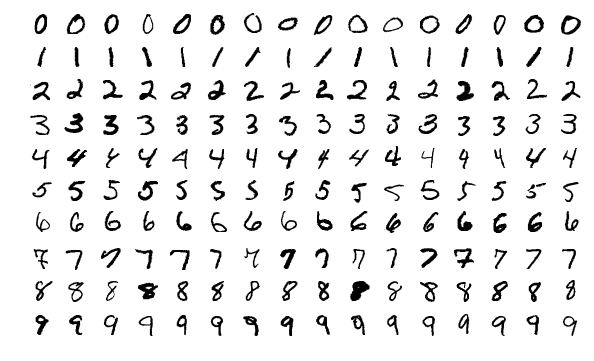
\includegraphics[width=\columnwidth]{img/MnistExamples.png}
        };
        \onslide<2->{
        \begin{scope}[x={(image.south east)},y={(image.north west)}]
          \draw[red,ultra thick] (0.22,0.15) rectangle (0.28,0.25);
        \end{scope}
        }
      \end{tikzpicture}
      \url{http://yann.lecun.com/exdb/mnist/index.html}
    \end{column}
  \end{columns}
\end{frame}
